\documentclass{beamer}
\usepackage[utf8]{inputenc}
\usepackage[T2A]{fontenc}
\usepackage[russian]{babel}
\usepackage[orientation=portrait,size=a0,scale=1.4]{beamerposter}
\usepackage{graphicx}
\usepackage{amsmath}
\usepackage{hyperref}
\usepackage{multicol}

\setbeamercolor{block title}{fg=white,bg=blue!70}
\setbeamercolor{block body}{fg=black,bg=blue!10}
\setbeamercolor{background canvas}{bg=white}

\title{Современные подходы в машинном обучении}
\author{Степанова Анна}
\institute{РГПУ им. А.И. Герцена}

\begin{document}

\begin{frame}
\centering
\vspace{-1cm}

\begin{columns}[t]

\begin{column}{0.30\textwidth}
\begin{block}{Введение}
\textbf{Актуальность:}
\begin{itemize}
\item Рост объёма данных
\item Развитие вычислительных мощностей
\item Появление новых алгоритмов
\end{itemize}
\vspace{0.2cm}
\textbf{Цель:}
\begin{itemize}
\item Сравнить эффективность методов
\item Определить области применения
\item Предложить рекомендации
\end{itemize}
\end{block}

\begin{block}{Методы}
\textbf{Классические:}
\begin{itemize}
\item Логистическая регрессия
\item Метод k-ближайших соседей
\item Наивный байесовский классификатор
\end{itemize}
\textbf{Современные:}
\begin{itemize}
\item Случайный лес
\item Градиентный бустинг
\item Глубокие нейронные сети
\end{itemize}
\end{block}
\end{column}

\begin{column}{0.35\textwidth}
\begin{block}{Результаты}
\begin{center}
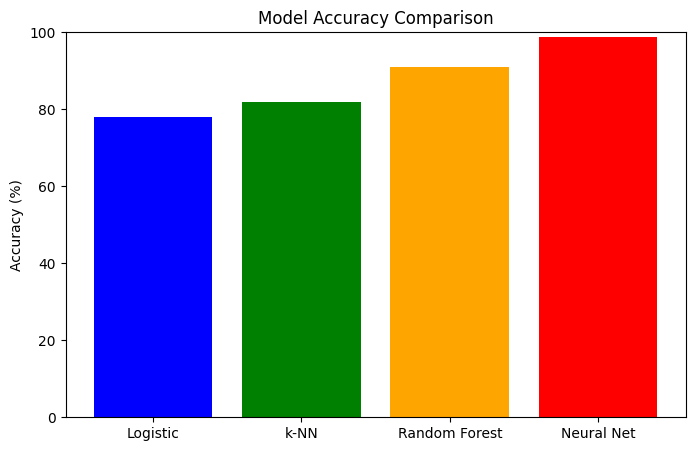
\includegraphics[width=0.85\linewidth]{gr1.png}
\par\small{График 1: Сравнение точности моделей}
\vspace{0.3cm}
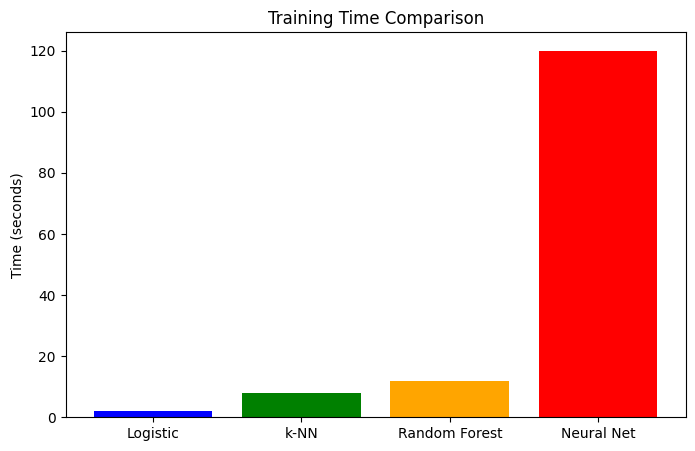
\includegraphics[width=0.85\linewidth]{gr2.png}
\par\small{График 2: Время обучения моделей}
\end{center}
\end{block}
\end{column}

\begin{column}{0.30\textwidth}
\begin{block}{Выводы}
\textbf{Лучшая точность:}
\begin{itemize}
\item Нейронные сети
\item 98.7\% на тестовых данных
\end{itemize}
\textbf{Быстрейшее обучение:}
\begin{itemize}
\item Случайный лес
\item 12 секунд
\end{itemize}
\textbf{Рекомендация:}
\begin{itemize}
\item Ансамблевые методы
\item Для больших данных -- нейросети
\end{itemize}
\end{block}

\begin{block}{Литература}
\begin{enumerate}
\item Bishop, C. M. (2006). Pattern Recognition and ML. Springer.
\item Goodfellow, I. et al. (2016). Deep Learning. MIT Press.
\item Hastie, T. et al. (2009). Elements of Statistical Learning. Springer.
\item Geron, A. (2019). Hands-On ML. O'Reilly.
\item Murphy, K. P. (2012). ML: A Probabilistic Perspective. MIT Press.
\end{enumerate}
\end{block}
\end{column}

\end{columns}

\end{frame}
\end{document}
